\let\negmedspace\undefined
\let\negthickspace\undefined
\documentclass[journal]{IEEEtran}
\usepackage[a5paper, margin=10mm, onecolumn]{geometry}
\usepackage{lmodern} % Ensure lmodern is loaded for pdflatex
\usepackage{tfrupee} % Include tfrupee package

\setlength{\headheight}{1cm} % Set the height of the header box
\setlength{\headsep}{0mm}     % Set the distance between the header box and the top of the text

\usepackage{gvv-book}
\usepackage{gvv}
\usepackage{cite}
\usepackage{amsmath,amssymb,amsfonts,amsthm}
\usepackage{algorithmic}
\usepackage{graphicx}
\usepackage{textcomp}
\usepackage{xcolor}
\usepackage{txfonts}
\usepackage{listings}
\usepackage{enumitem}
\usepackage{mathtools}
\usepackage{gensymb}
\usepackage{comment}
\usepackage[breaklinks=true]{hyperref}
\usepackage{tkz-euclide} 
\usepackage{listings}
\def\inputGnumericTable{}                                 
\usepackage[latin1]{inputenc}                                
\usepackage{color}                                            
\usepackage{array}                                            
\usepackage{longtable}                                       
\usepackage{calc}                                             
\usepackage{multirow}                                         
\usepackage{hhline}                                           
\usepackage{ifthen}                                           
\usepackage{lscape}

\begin{document}

\bibliographystyle{IEEEtran}
\vspace{3cm}

\title{9.6.9}
\author{EE24BTECH11002 - Agamjot Singh}
% \maketitle
% \newpage
% \bigskip
{\let\newpage\relax\maketitle}

\renewcommand{\thefigure}{\theenumi}
\renewcommand{\thetable}{\theenumi}
\setlength{\intextsep}{10pt} % Space between text and floats

\textbf{Question:}
\newline
Solve the differential equation:
\begin{align}
    x\frac{dy}{dx} + y - x + xy \cot{x} = 0 \text{ , } x\neq 0\\
\end{align}

\textbf{Theoritical solution:}
The given equation is a linear ordinary differential equation.
\begin{align}
    \frac{dy}{dx} + \frac{y}{x} - 1 + y \cot{x} = 0\\
    \frac{dy}{dx} + y \brak{\frac{1}{x} + \cot{x}} = 1
\end{align}
The integrating factor is given by 
\begin{align}
    e^{\int \brak{\frac{1}{x} + \cot{x}} \, dx} &= e^{\log \brak{x \sin{x}}}\\
                                                &= x \sin {x}
\end{align}
Multiplying on both sides, we get,
\begin{align}
    x\sin{x}\frac{dy}{dx} + y\brak{\sin{x} + x\cos{x}} &= x\sin{x}\\
    d\brak{y x\sin{x}} &= x\sin{x} \, dx
\end{align}
Integrating on both sides, we get,
\begin{align}
    y x\sin{x} &= \int x\sin{x} \, dx\\
               &= -x\cos{x} + \sin{x} + C \text{, where } C \text{ is the constant of integration}\\
    \implies y &= y\brak{x} = -\cot{x} + \frac{1}{x} + \frac{C}{x\sin{x}}
\end{align}

\textbf{Computational Solution:} Euler's method
\newline
By the first principle of derivative,
\begin{align}
    y^{\prime}\brak{x} &= \lim_{h\to0} \frac{y\brak{x + h} - y\brak{x}}{h}\\
    y\brak{x + h} &= y\brak{x} + h\brak{y^{\prime}\brak{x}} \text{, } h\to0
\end{align}
Expressing this system in an iterative format \brak{\text{by method of finite differences}},
\begin{align}
    y\brak{x_{n + 1}} &= y\brak{x_n} + hy^{\prime}\brak{x_n}\\
    y_{n + 1} &= y_n + hy^{\prime}\brak{x_n}\\
    x_{n + 1} &= x_n + h
\end{align}
Substituting the value of $y^{\prime}\brak{x}$, we get,
\begin{align}
    y_{n + 1} &= y_n + h\brak{1 - y_n\brak{\frac{1}{x_n} + \cot{x_n}}}
\end{align}

For iteratively plotting the above system, we only take $3$ intervals as the value tends to infinity at infinitely many points, thus we take $3$ initial conditions,
\begin{align}
    \brak{x_0}_1 = 0.21 \text{ , } \brak{y_{1, 0}}_1 = 22\\
    \brak{x_0}_2 = 3.2 \text{ , } \brak{y_{1, 0}}_2 = -20\\
    \brak{x_0}_3 = -3.1 \text{ , } \brak{y_{1, 0}}_3 = -20
\end{align}
we get the following plot.

\begin{figure}[h!]
   \centering
   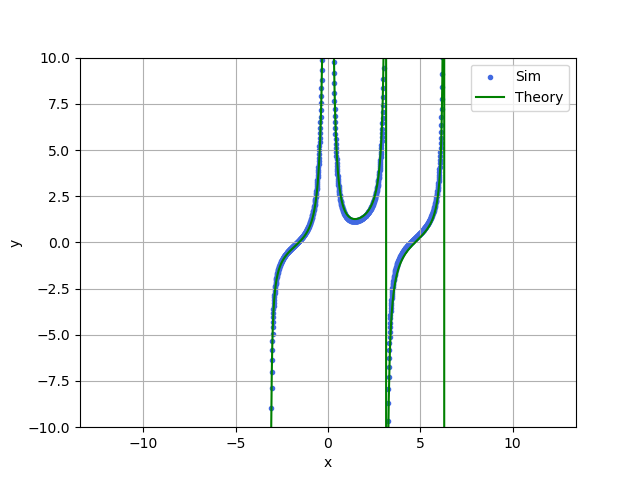
\includegraphics[width=0.7\columnwidth]{figs/graph.png}
    \caption{Computational solution for $xy^{\prime} + y - x + xy\cot{x} = 0$}
   \label{label}
\end{figure}

\end{document}
